\documentclass[10pt]{article}
\usepackage[export]{adjustbox}
\usepackage{amsmath}
\usepackage{array}
\usepackage[makeroom]{cancel}
\usepackage{chemfig}
\usepackage{enumitem}
\usepackage{float}
\usepackage{graphicx}
%Load mhchem using some package options
\usepackage[version=4]{mhchem}
\usepackage{multicol}
\usepackage{siunitx}

\title{
    Problem Set \#11
    \\  \small
    CHEM101A: General College Chemistry
    }
\author{Donald Aingworth}
\date{October 31, 2025}

\newcommand{\E}[1]{\times 10^{#1}}
\newcommand{\hc}{1.9864748\E{-25}\,\unit{\joule\,\meter}}
\newcommand{\U}[1]{\underline{#1}}

\begin{document}
    \DeclareSIUnit{\atm}{atm}
    \DeclareSIUnit{\molarity}{M}
    \DeclareSIUnit{\M}{M}
    \DeclareSIUnit{\torr}{torr}

    \maketitle

    % \setcounter{section}{22}

    \pagebreak
    \section{Topic F Problem 1}
        Draw a bond energy diagram (a graph of potential energy versus distance between the nuclei) for the bond in \ce{O2}, which has a bond energy of 495 kJ/mol and a bond distance of 121 pm.
        
        \subsection{Solution}

    \pagebreak
    \section{Topic F Problem 2}
        Draw Lewis structures for each of the following molecules. 
        For each molecule, the first atom in the formula is the central atom and all other atoms are bonded to it.
        \begin{multicols}{3}
            \begin{enumerate}[label=\alph*)]
                \item   \ce{CH4}
                \item   \ce{PCl3}
                \item   \ce{PBr5}
                \item   \ce{COF2}
                \item   \ce{SOF2}
                \item   \ce{SeF4}
            \end{enumerate}
        \end{multicols}
        
        \subsection{Solution}


    \pagebreak
    \section{Topic F Problem 3}
        Draw Lewis structures for each of the following polyatomic ions. 
        If there are multiple resonance structures for an ion, you only need to draw one of the resonance structures.
        \begin{multicols}{3}
            \begin{enumerate}[label=\alph*)]
                \item   \ce{NO2-}
                \item   \ce{NH4+}
                \item   \ce{BF4-}
                \item   \ce{CO3^2-}
                \item   \ce{CN-}
                \item   \ce{O2^2-}
                \item   \ce{ClO4-}
                \item   \ce{SeO4^2-}
                \item   \ce{IF4-}
            \end{enumerate}
        \end{multicols}
        
        \subsection{Solution}


    \pagebreak
    \section{Topic F Problem 4}
        Consider each of the following molecules:
        \begin{center}
            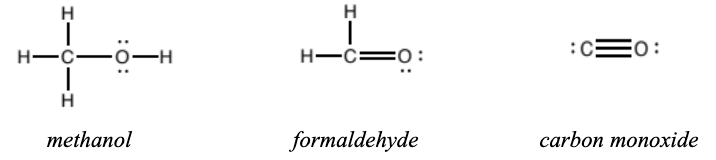
\includegraphics[width=0.75\textwidth]{img-F4.png}
        \end{center}
        \begin{enumerate}[label=\alph*)]
            \item   What is the bond order of the carbon-oxygen bond in each molecule?
            \item   Which molecule has the largest carbon-oxygen bond energy?
            \item   Which molecule has the largest carbon-oxygen bond distance?
            \item   Would you expect the carbon-hydrogen bond distances in methanol and formaldehyde to be equal, or will they be significantly different? 
                If they are different, which molecule should have the larger C-H bond distances?
        \end{enumerate}
        
        \subsection{Solution}


    \pagebreak
    \section{Topic F Problem 5}
        For each of the bond types in parts a through d below, answer the following questions. 
        You may refer to the table of electronegativity values in the textbook.
        \begin{itemize}
            \item   Are these bonds polar?
            \item   If they are polar, which atom is positively charged (if any)?
        \end{itemize}
        \begin{multicols}{2}
            \begin{enumerate}[label=\alph*)]
                \item   The \ce{C-Cl} bonds in \ce{CCl4}
                \item   The \ce{O-Cl} bonds in \ce{OCl2}
                \item   The \ce{C-H} bonds in \ce{CH4} 
                \item   The \ce{C-C} bond in \ce{C2H6}
            \end{enumerate}
        \end{multicols}
        
        \subsection{Solution}


    \pagebreak
    \section{Topic F Problem 6}
        Using the bond dissociation energy values in the text, calculate an approximate value of $\Delta$H for the reaction: \ce{N2 (g) + 3 H2 (g) -> 2 NH3 (g)}.
        
        \subsection{Solution}


    \pagebreak
    \section{Topic F Problem 7}
        Xenon is one of the “inert gases”, but it can form a number of compounds, including xenon trioxide (XeO3). 
        When heated, xenon trioxide breaks down explosively into the elements:
        \begin{center}
            \ce{2 XeO3 (g) -> 2 Xe (g) + 3 O2 (g), \Delta H = -804\unit{\kilo\joule}}
        \end{center}
        Use this value and the bond dissociation energy for the bond in O2 to calculate a value for the xenon-oxygen bond energy. Give your answer in kJ/mol.
        
        \subsection{Solution}


    \pagebreak
    \section{Topic F Problem 8}
        For each of the following molecules, determine the formal charge on each atom. 
        (In your answer, draw the Lewis structure and write all non-zero formal charges next to the corresponding atoms.)
        \begin{center}
            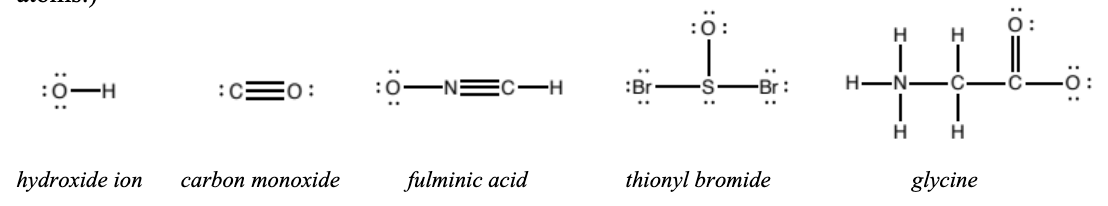
\includegraphics[width=\textwidth]{img-F8.png}
        \end{center}
        
        \subsection{Solution}


    \pagebreak
    \section{Topic F Problem 9}
        There are two resonance structure for the ozone molecule, \ce{O3}; these structures are shown below.
        \begin{center}
            \begin{multicols}{2}
                \begin{figure}[H]
                    \centering
                    \chemfig{\charge{180=\:,90=\:,-90=\:}{O} - \charge{-90=\:}{O} = \charge{0=\:,-90=\:}{O}}
                    \caption{Structure \#1}
                \end{figure}
                
                \begin{figure}[H]
                    \centering
                    \chemfig{\charge{180=\:,-90=\:}{O} = \charge{-90=\:}{O} - \charge{0=\:,90=\:,-90=\:}{O}}
                    \caption{Structure \#2}
                \end{figure}
            \end{multicols}
        \end{center}

        \begin{enumerate}[label=\alph*)]
            \item   A student says “sometimes each bond in \ce{O3} is the same strength as the bond in O=O, and sometimes it's the same strength as the central bond in H-O-O-H.” 
                Is this an accurate statement? 
                Explain your answer.
            \item   Another student says “when \ce{O3} looks like structure \#1, the bond on the left is longer than the bond on the right.” 
                Is this an accurate statement? 
                Explain your answer.
        \end{enumerate}
        
        \subsection{Solution}
            \begin{enumerate}[label=\alph*/]
                \item   This is not accurate. In truth, the bond strength does not alternate, it stays the same at all times. The difference is that the bond strength is stronger than the H-O-O-H bond but weaker than the O=O bond.
                \item   This is not accurate. Firstly, the structure of \ce{O3} does not look like either at any given time. Secondly, the two bonds are identical in both strength and length. If \ce{O3} were to look like structure \#1, it would have a longer bond on the left than on the right, but that is not the case and so is the conclusion that arises from it.
            \end{enumerate}


    \pagebreak
    \section{Topic F Problem 10}
        This problem asks you to compare two ions: \ce{NO2+} and \ce{NO2-}. 
        In both of these ions, the nitrogen is the central atom.
        \begin{enumerate}[label=\alph*)]
            \item   One of these ions requires two resonance structures to represent it accurately. Which one is it? Draw the two reasonable resonance structures for this ion.
            \item   For the other ion, there are three resonance structures that satisfy the octet rule. Draw these three resonance structures for this ion.
            \item   The ion in part b actually requires just one Lewis structure to depict it accurately. Which structure is this, and why is this the only structure you need?
            \item   Which are shorter: the nitrogen-oxygen bond distances in \ce{NO2+}, or the nitrogen-oxygen bond distances in \ce{NO2-}? Or do the two ions have equal N–O bond distances? Explain your answer.
        \end{enumerate}
        
        \subsection{Solution}

    \pagebreak
    \setcounter{section}{14}
    \section{Topic F Problem 15}
        What are the approximate values (in degrees) for the bond angles labeled A through E in the molecule below?
        \begin{center}
            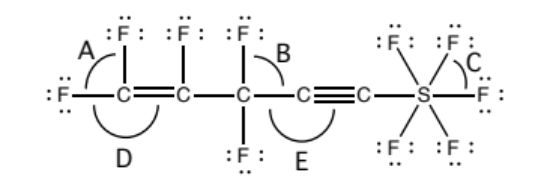
\includegraphics[width=0.7\textwidth]{img-F15.png}
        \end{center}
        
        \subsection{Solution}
            \begin{enumerate}[label=\Alph*:]
                \item   120\unit{\degree}
                \item   109.5\unit{\degree}
                \item   90\unit{\degree}
                \item   120\unit{\degree}
                \item   180\unit{\degree}
            \end{enumerate}

    \pagebreak
    \setcounter{section}{20}
    \section{Topic F Problem 21}
        Questions a through d (on the next page) refer to the molecule below.
        \begin{center}
            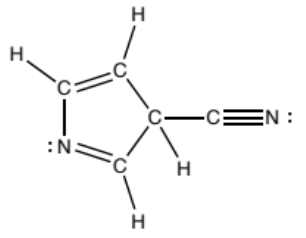
\includegraphics[width=0.3\textwidth]{img-F21.png}
        \end{center}

        \begin{enumerate}[label=\alph*)]
            \item   How many sigma bonds and how many pi bonds are there in this molecule?
            \item   What atomic orbitals form the carbon-nitrogen double bond? Tell whether each orbital is involved in a sigma bond or a pi bond.
            \item   What atomic orbitals form the carbon-nitrogen triple bond? Tell whether each orbital is involved in a sigma bond or a pi bond.
            \item   What atomic orbitals contain the nonbonding electrons?
        \end{enumerate}
        
        \subsection{Solution}

    \pagebreak
    \tableofcontents
\end{document}